\section{Motivation}
It was noticed that the critical pressure and temperature plot for cavitation of electron bubbles in liquid helium deviated from theoretical predictions at low temperatures in thickness mode. Nonlinear propagation of sound might be able to explain these experimental anomalies. The experimental data also suggests that if a linear fit were to be made, a certain static pressure alone is enough to produce the required negative pressure at the focus. This cannot be possible since, in the absence of driving, the pressure at the focus should be equal to the static pressure. The extrapolation gave a different pressure suggesting that some nonlinear calculations must be done in order to find the correct critical pressure for the bubble to burst.

We investigate whether the nonlinear propagation of the sound can be modeled using simulations and whether we can calculate the pressure at the focus due to the sound wave. To do this, we ran simulations to estimate the nonlinearity at two different frequencies, thickness mode (high frequency) and flexure mode (low frequency). We would like to know whether the relationship between the threshold voltage and the static pressure is nonlinear.

Understanding the propagation of sound in liquid helium will be crucial in future experiments concerning exotic ions since the exact pressure at the focus on the transducer needs to be known. We also need to know the consequences of using thickness mode for experiments.

\section{Background}

B.M. Abraham et al. proposed a Taylor series expansion of pressure: \cite{PhysRevA.2.550.3}

\begin{equation}\label{preseq1}
P = (\rho - \rho_0) \left.\frac{\partial P}{\partial \rho}\right|_0 + \frac{1}{2}(\rho - \rho_0)^2 \left.\frac{\partial^2 P}{\partial \rho^2}\right|_0 + \frac{1}{6}(\rho - \rho_0)^3 \left.\frac{\partial^3 P}{\partial \rho^3}\right|_0 + ...
\end{equation}

and found that\\

$\left.\frac{\partial P}{\partial \rho}\right|_0$ = c$_0^2$, $\left.\frac{\partial^2 P}{\partial \rho^2}\right|_0$ = $\frac{2c_0^2\mu_0}{\rho_0}$ and $\left.\frac{\partial^3 P}{\partial \rho^3}\right|_0$ = $\frac{2c_0^2\mu_0}{\rho_0}$ + $\frac{2c_0^2w_0}{\rho_0}$\\

The constants $\rho_0$ and $c_0$ are the density and sound velocity at zero pressure, respectively. The constant $\mu_0$ is known as the Gruneisen Constant. B.M. Abraham et al \cite{PhysRevA.2.550.3} found the Gruneisen Constant in liquid helium to be $2.84$. The experiment was made in the vicinity of $0.5$ K. They also found that $w_0$, another experimental constant, is $0.194$.

This Taylor series expansion can be used to simulate the propagation of sound in liquid helium. We will consider the first three terms in our calculations. In the simulations, the traducer wall was driven as:

\begin{equation}\label{diseq}
u_t = u_0 sin(\omega t)(1-e^{\frac{-t}{\tau}})
\end{equation}
Where $u_0$ is the initial displacement of the wall and $u_t$ is the displacement at time $t$. $u_0$ is proportional to the voltage applied to the transducer. $\tau$ is the time needed for the transducer amplitude to build up. The equation models the build up of sound well because we require the amplitude of the pressure to increase linearly for a short time. This can be achieved by Eq. \ref{diseq} since from the first order Taylor series expansion of $e^{\frac{-t}{\tau}}$, for small t:
$$1-e^{\frac{-t}{\tau}} \approx 1 - 1 + \frac{-t}{\tau}  \approx \frac{-t}{\tau}$$
This means that at the peaks, where $sin(\omega t)$ is equal to $1$, the amplitude should increase linearly. For larger times, the exponential term will die out and the oscillations would be sinusoidal. Finally, differentiating Eq. \ref{diseq} with respect to time would yield the velocity. 

\section{Simulation Algorithm}
First, an array with various values of $r$, the number of which depend on the impute parameters, is created from $r = 0$ to $r = 0.8$ cm (which is the distance of focus from the transducer). As the program loops through the time, each value of $r$ is assigned a corresponding density which is given by the following relations:

\begin{equation}\label{radeq1}
Vol_{intl} = \frac{4}{3}\pi [(r_{n+1})^3 - (r_n)^3]
\end{equation}

\begin{equation}\label{radeq2}
Vol_r = \frac{4}{3}\pi [(r_{n+1} + u_{t+1})^3 - (r_n + u_t)^3]
\end{equation}

\begin{equation}\label{deneq1}
\rho_r = \rho_{intl} \frac{Vol_{intl}}{Vol_r}
\end{equation}

$Vol_{intl}$ is the initial volume between $r = r_n$ and $r_{n+1}$.Thus the $nth$ value of $Vol_{intl}$ is the volume of the shell between the $(n+1)th$ value of $r$ and $(n+1)th$ value of $r$. Similarly, $Vol_n$ is volume of the shell between the $nth$ value of $r$ and $(n+1)th$ value of $r$ when the sound wave is going through the liquid. $\rho_{intl}$ is the density of helium at a given static pressure. Therefore being constant throughout the experiment. Due to the propagation of the sound wave, the displacement of the wave at a given point must be added to the corresponding value of $r$ in order to find the correct value of $Vol_r$. The instantaneous density of the liquid $\rho_r$, at radius $r$, is calculated using Eq. \ref{deneq1}. Finally, the corresponding pressure $P$, at radius $r$ and time $t$, is calculated from $\rho_r$ using Eq. \ref{preseq1} setting $\rho$ = $\rho_r$.

\section{Results}

The pressure at the focus was plotted against time in Fig. \ref{presvstime} for both resonant frequencies. The static pressure in each case was $1.0$ atm. The initial straight line, indicating the time sound needs to reach the focus, agrees with what one would expect using the velocity of sound in liquid helium and the radius of focus.
\begin{figure}[H]
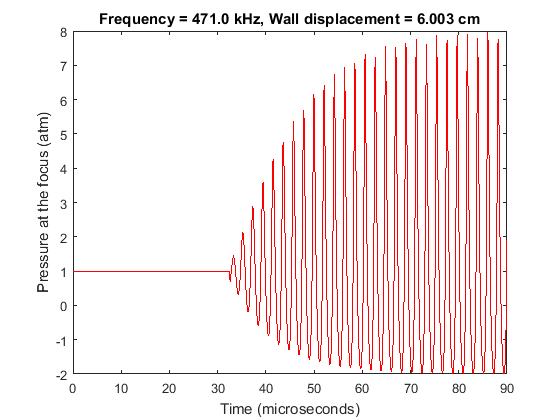
\includegraphics[width=75mm, height=60mm]{Nonlinear_correction/pvt_hf.png}
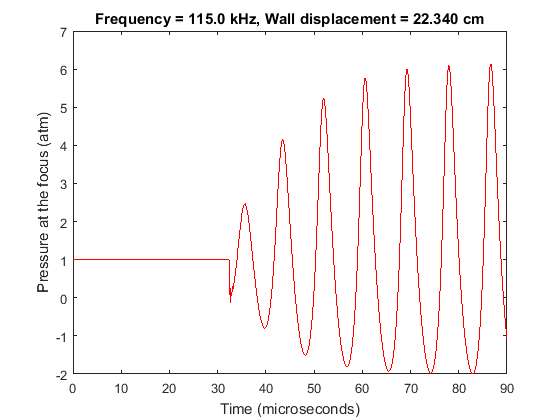
\includegraphics[width=75mm, height=60mm]{Nonlinear_correction/pvt_lf.png}
\caption{Pressure versus Time plots for the focus.}
\label{presvstime}
\end{figure}
Figure \ref{presvsrad} shows the pressure vs radius plot. $r=0$ corresponds to the focus. The static pressure was $1.0$ atm. The plot shows that pressure at focus (where $r=0$) is the maximum. The transducer is hemispherical. Therefore, the focus is equidistant from all point on the transducer. Thus the sound waves convergence at the focus interfering constructively. This is because they all have the same phase.
\begin{figure}[H]
\centering 
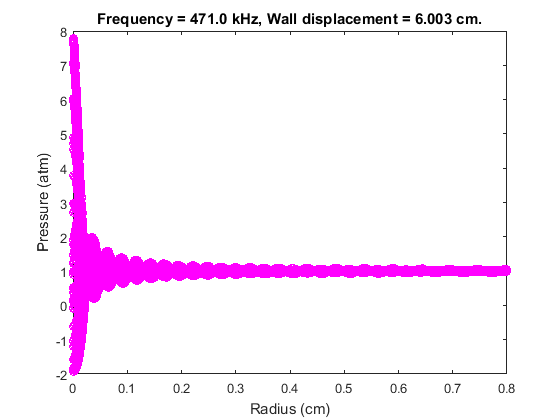
\includegraphics[width=75mm, height=60mm]{Nonlinear_correction/prevsrad.png}
\caption{Pressure versus time plots for the focus.}
\label{presvsrad}
\end{figure}

Ultimately, the goal was to find the displacement of the wall that gives a pressure of -2 atm at the focus. This was done by varying the initial amplitude of the wall, keeping the static pressure constant. The initial density for a given static pressure was found by solving Eq. \ref{preseq1} for $\rho$. A plot of displacement of the wall versus static pressure is shown in Fig. \ref{disvspress}. The third plot in Fig. \ref{disvspress} shows the same relations, but with minimum pressure at the focus being $-1$ atm.

\begin{figure}[H]
\begin{tabular}{cc}
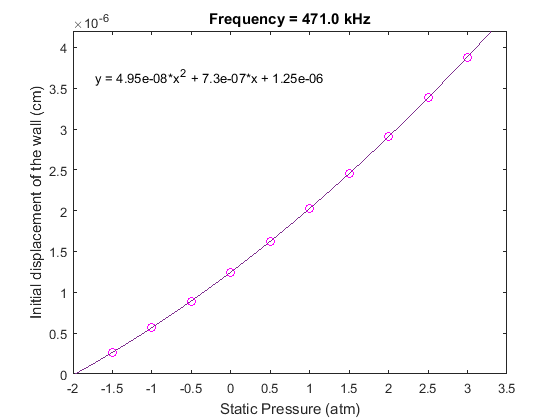
\includegraphics[width=75mm, height=60mm]{Nonlinear_correction/p_-2_hf.png} 
& 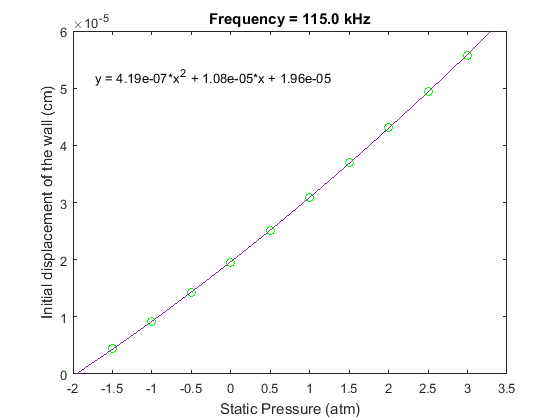
\includegraphics[width=75mm, height=60mm]{Nonlinear_correction/p_-2_lf.png}\\
\multicolumn{2}{c}{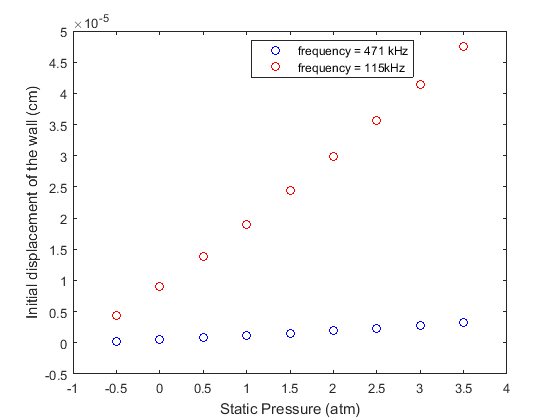
\includegraphics[width=75mm, height=60mm]{Nonlinear_correction/p-minus1.png}}\\
\end{tabular}
\caption{Displacement versus static pressure plots.}
\label{disvspress}
\end{figure}

The plot of displacement verses static pressure was found to be non linear. This means that the nonlinear propagation of sound must have impacted the pressure-temperature plot in Chapter 2. It was also observed that the nonlinear effects were more prominent at high frequency. This also agrees with the experiment since the anomalies were found to be significant at high frequency. The displacement versus pressure relations can used for calculations. A quadratic linear fit has been included in Fig. \ref{disvspress}. Ideally the curve should have passed through $(-2,0)$ and $(-1,0)$ for a static pressure of $-2$ atm and $-1$ atm respectively; however, the fit came really close to those points. 

Thus the simulation was quite successful in modeling the propagation of sound waves in the liquid. The most basic requirement was that the pressure at the focus should be higher than any point in the liquid. It was also expected that the amplitude of the pressure should increase linearly for a short time. Both of these requirements were satisfied. We also concluded that the propagation of sound in liquid helium is indeed nonlinear. This type of calculation can form a basis for future experiments involving exotic ions.

